
\begin{picture} (270.000000,185.771429)(0,0)
\put(0.0, 0.0){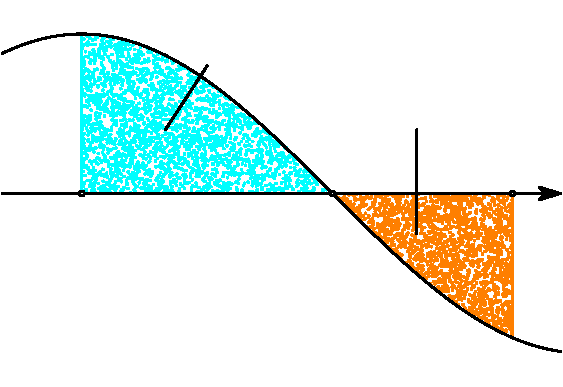
\includegraphics{figures/08Integral-posandneg.pdf}}
    \put(101.42, 156.14){\sffamily\itshape Area $=A_1>0$}
    \put(171.46, 125.51){\sffamily\itshape Area $=A_2>0$}
    \put( 39.29,  80.89){\sffamily\itshape $a$}
    \put(244.03,  96.89){\sffamily\itshape $b$}
    \put(159.56,  96.89){\sffamily\itshape $c$}
    \put( 23.97,  39.29){\sffamily\itshape $\int_a^b f(x)dx = A_1 - A_2$}
\end{picture}
